\documentclass[aps,twocolumn,prd,showpacs,showkeys,preprintnumbers,superscriptaddress,nobibnotes,floatfix,longbibliography]{revtex4-1}

\pdfoutput=1

\usepackage{amsmath}
\usepackage{amsfonts}
\usepackage{amssymb}
\usepackage{mathrsfs}
\usepackage{graphicx}
\usepackage{color}
\usepackage{longtable}
\usepackage{bm}
\usepackage{hyperref}
% \usepackage{blindtext}
% \usepackage{wasysym}


\newcommand{\ie}{{\it i.e.}}
\newcommand{\Ie}{{\it I.e.}}
\newcommand{\eg}{{\it e.g.}}
\newcommand{\Eg}{{\it E.g.}}
\newcommand{\cf}{{\it cf.}}
\newcommand{\etc}{{\it etc.}}
\newcommand{\eq}{Eq.}
\newcommand{\eqs}{Eqs.}
\newcommand{\Def}{Definition}
\newcommand{\fig}{Fig.}
\newcommand{\Fig}{Fig.}
\newcommand{\figs}{Figures}
\newcommand{\Figs}{Figures}
\newcommand{\Ref}{Ref.}
\newcommand{\Refs}{Refs.}
\newcommand{\Sec}{Section}
\newcommand{\Secs}{Sections}
\newcommand{\App}{Appendix}
\newcommand{\Apps}{Appendices}
\newcommand{\Tab}{Tab.}
\newcommand{\Tabs}{Tabs.}
\newcommand\brabar{\raisebox{-2.0pt}{\scalebox{.2}{ \textbf{(}}}\raisebox{-2.0pt}{{\_}}\raisebox{-2.0pt}{\scalebox{.2}{\textbf{ )}}}}

\newcommand{\equ}[1]{\eq~(\ref{equ:#1})}
\newcommand{\figu}[1]{\fig~\ref{fig:#1}}
\newcommand{\tabl}[1]{\Tab~\ref{tab:#1}}
\newcommand{\bi}{\begin{itemize}}
\newcommand{\ei}{\end{itemize}}
\newcommand{\ra}{\rightarrow}

\newcommand{\matr}[1]{\mathbf{#1}} 

\newcommand{\MB}[1]{{\color{blue}[{\bf MB:} #1]}}
\newcommand{\CR}[1]{{\color{red}[{\bf CR:} #1]}}
\newcommand{\IT}[1]{{\color{magenta}[{\bf IT:} #1]}}

\begin{document}
 
\title{Notes on secret interactions of high-energy astrophysical neutrinos} 

\author{Charlotte Rosenstroem}
\email{vkc652@alumni.ku.dk}
\affiliation{Niels Bohr International Academy and DARK, Niels Bohr Institute, Blegdamsvej 17, 2100 Copenhagen, Denmark}
% \thanks{ORCID: \href{http://orcid.org/0000-0001-6923-0865}{0000-0001-6923-0865}}

\author{Mauricio Bustamante}
\email{mbustamante@nbi.ku.dk}
\affiliation{Niels Bohr International Academy and DARK, Niels Bohr Institute, Blegdamsvej 17, 2100 Copenhagen, Denmark}
\thanks{ORCID: \href{http://orcid.org/0000-0001-6923-0865}{0000-0001-6923-0865}}

\author{Irene Tamborra}
\email{tamborra@nbi.ku.dk}
\affiliation{Niels Bohr International Academy and DARK, Niels Bohr Institute, Blegdamsvej 17, 2100 Copenhagen, Denmark}
\thanks{ORCID: \href{http://orcid.org/0000-0001-7449-104X}{0000-0001-7449-104X}}

% \preprint{v1}

\date{\today}

\begin{abstract}
 Notes on the calculation of secret interactions of high-energy astrophysical neutrinos with the low-energy relic neutrino background.
\end{abstract}

%\pacs{14.60.Pq}
%\keywords{Neutrino mass and mixing, Beta beams}

\maketitle

%%%%%%%%%%%%%%%%%%%%%%%%%%%%%%%%%%%%%%%%%%%%%%%%%%%%%%%%%%%%%%%%%%%%%%%%%%%%%%%
%%%%%%%%%%%%%%%%%%%%%%%%%%%%%%%%%%%%%%%%%%%%%%%%%%%%%%%%%%%%%%%%%%%%%%%%%%%%%%%


\section{Introduction}\label{section:introduction}

The existence of a new mediator that couples to neutrinos may have observable consequences for the flux of high-energy astrophysical neutrinos that IceCube measures.  The new mediator may enhance the interaction between TeV--PeV astrophysical neutrinos and meV neutrinos from the relic neutrino background (C$\nu$B).  For some values of the mass of the new mediator, the interaction could be resonant within the energy range observed by IceCube.  If the interaction is elastic, its presence could manifest in the IceCube energy spectrum as a dip --- at the resonance energy --- and a pile-up of neutrinos at lower energy\ \cite{Ng:2014pca, Ioka:2014kca, Ibe:2014pja, DiFranzo:2015qea}

In this project, we explore whether there are signs of such interaction in the energy spectrum of high-energy astrophysical neutrinos reported by IceCube.  Later, we might also consider effects on their flavor composition.

In these notes, we outline the theory and computation of the effects of the new $\nu \nu$ interaction, and the comparison to IceCube results.


%%%%%%%%%%%%%%%%%%%%%%%%%%%%%%%%%%%%%%%%%%%%%%%%%%%%%%%%%%%%%%%%%%%%%%%%%%%%%%%
%%%%%%%%%%%%%%%%%%%%%%%%%%%%%%%%%%%%%%%%%%%%%%%%%%%%%%%%%%%%%%%%%%%%%%%%%%%%%%%


\section{The neutrino-neutrino cross section}\label{section:cross_section}

We consider new interactions between the neutrino mass eigenstates $\nu_i$ ($i=1,2,3$) of the astrophysical neutrino flux and the relic neutrino background.  We assume that the coupling constant between the neutrino and the new mediator is the same for all mass eigenstates, \ie, $g_i \equiv g$, $\forall i$.  We also assume that all of the neutrino mass eigenstates have the same mass, $m_\nu$  \MB{What value?}. Later, to consider effects on the flavor composition, we may drop these two assumptions and generalize the formalism, as in, \eg, \Refs\ \cite{Farzan:2014gza, DiFranzo:2015qea}.

%%%%%%%%%%%%%%%%%%%%%%%%%%%%%
\begin{figure}[t!]
 \centering
 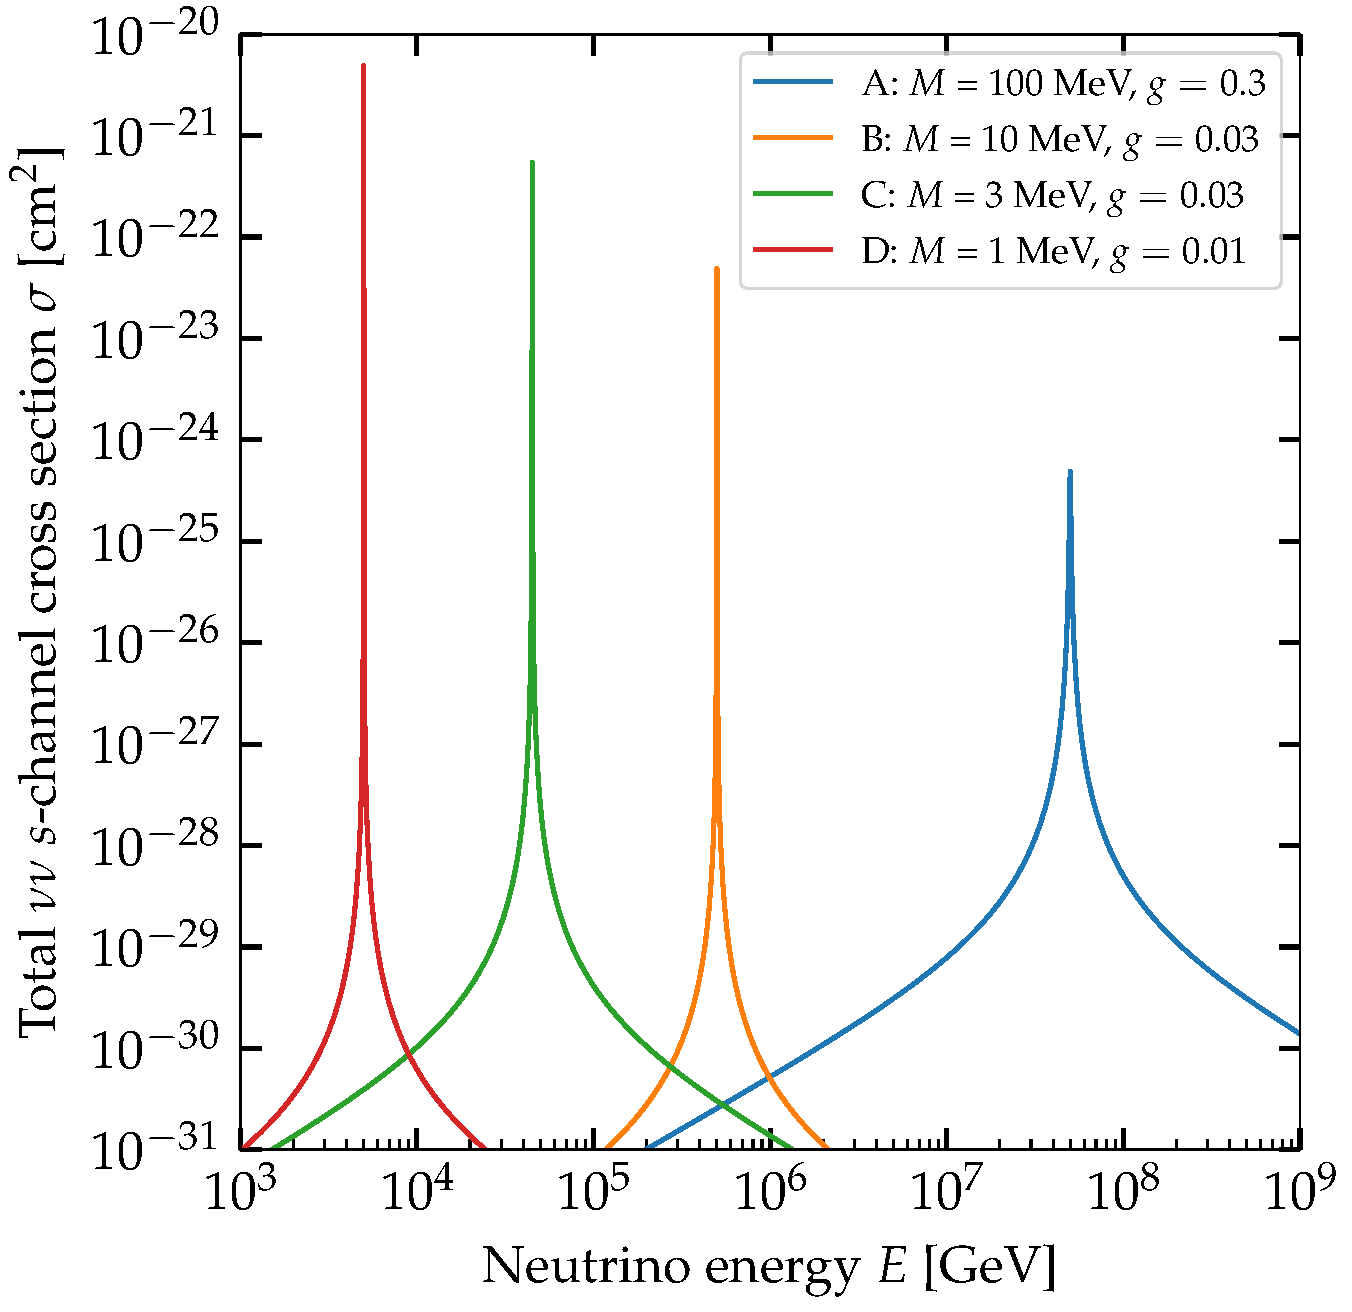
\includegraphics[width=\columnwidth]{cs_nu_nu_s_channel_scalar.pdf}
 \caption{\label{fig:total_cs_s_channel_scalar}Total cross section of the $\nu\nu$ interaction in the $s$-channel, for a scalar mediator.  The benchmark points A--D are the same as in \Ref\ \cite{Ng:2014pca}.}
\end{figure}
%%%%%%%%%%%%%%%%%%%%%%%%%%%%%

As a start, we consider a scalar mediator.  We consider only the $s$-channel contribution to the cross section; the $t$-channel is heavily suppressed in comparison\ \cite{Ng:2014pca, Farzan:2014gza}.  Below, we assume that there is only one resonance in the energy window of our interest.  Thus, the cross section of $\nu \nu$ interactions has a Breit-Wigner form,
\begin{equation}
 \sigma(E)
 =
 \frac{g^4}{4\pi}
 \frac{s}{\left(s-M^2\right)^2+M^2\Gamma^2} \;,
\end{equation}
where $s = 2 E m_\nu$, $E$ is the neutrino energy, $M$ is the mass of the mediator, and $\Gamma = g^2 M / (4\pi)$ is the decay width of the mediator. 

Figure \ref{fig:total_cs_s_channel_scalar} shows the cross section as a function of energy, for selected benchmark scenarios.

To include the effect the $\nu \nu$ interactions on the flux of high-energy astrophysical neutrinos, we need the differential cross section.  Because the mediator is a scalar, it decays isotropically in its rest frame.  As a result, for an incoming neutrino with energy $E$ and outgoing neutrino with energy $E^\prime$, the energy distribution of the outgoing neutrino is uniform within the energy range $E_{\min} \leq E^\prime \leq E$, where $E_{\min} = m_\nu E / (2E+m_\nu)$.  Thus the differential cross section is
\begin{equation}
 \frac {{\rm d}\sigma} {{\rm d}E} (E, E^\prime)
 =
 \sigma(E)
 \frac { \theta(E-E^\prime) } { E-E_{\min} }
 \theta( E^\prime-E_{\min}) \;,
\end{equation}
where $\theta$ is the step function.  \MB{An alternative form of the differential cross section is the one immediately following Eq.~(8) in \Ref\ \cite{DiFranzo:2015qea}.}


%%%%%%%%%%%%%%%%%%%%%%%%%%%%%%%%%%%%%%%%%%%%%%%%%%%%%%%%%%%%%%%%%%%%%%%%%%%%%%%
%%%%%%%%%%%%%%%%%%%%%%%%%%%%%%%%%%%%%%%%%%%%%%%%%%%%%%%%%%%%%%%%%%%%%%%%%%%%%%%


\section{The flux of high-energy astrophysical neutrinos}

At time $t$, we describe the neutrino beam via the comoving number density of neutrinos $n(t)$ (in units of cm${-3}$).  Its energy-differential is $\tilde{n}(t, E) = {\rm d} n(t,E) / {\rm d} E$ (in units of cm$^{-3}$ GeV$^{-1}$).  Thus, the neutrino flux at Earth (in units of GeV$^{-1}$ cm$^{-2}$ s$^{-1}$ sr$^{-1}$) is
\begin{equation}
 J(E)
 \equiv
 \frac {{\rm d} N} {{\rm d}E ~{\rm d}A ~{\rm d}t ~{\rm d}\Omega}
 =
 \frac{c}{4\pi} \tilde{n}(0,E) \;.
\end{equation}
Here and in what follows we adopt the notation from \Ref\ \cite{Ng:2014pca}, which is widely used.

To compute the effect of $\nu \nu$ interactions on the flux of high-energy astrophysical neutrinos, we solve the propagation equation 
\begin{widetext}
 \begin{equation}\label{equ:prop_eq}
  \frac {\partial \tilde{n}(t,E)} {\partial t}
  =
  \frac {\partial} {\partial E} \left( b(t,E) \tilde{n}(t,E) \right)
  + \mathcal{L}(t, E)
  - c n_t(t) \sigma(E) \tilde{n}(t,E)
  + c n_t(t) \int_E^\infty dE^\prime \tilde{n}(t,E^\prime) \sum_j \frac {{\rm d} \sigma_j} {{\rm d}E} \;,
 \end{equation}
\end{widetext}
with $E$ the neutrino energy at time $t$.  For simplicity, we recast this equation instead in terms of redshift by using the relation between time and redshift\ \cite{Hogg:1999ad}, \ie, ${\rm d}t/{\rm d}z = -\left[ (1+z) H(z) \right]^{-1}$.  Here, $H(z) \simeq H_0 \sqrt{\Omega_\Lambda + \Omega_m(1+z)^3}$ is the Hubble parameter, where $H_0 = 100 h$ km s$^{-1}$ Mpc$^{-1}$ = $h \times (9.777752~\text{Gyr})^{-1}$ is the Hubble constant, with $h = 0.678$, and $\Omega_\Lambda = 0.692$ and $\Omega_m = 0.308$ are the adimensional energy densities of vacuum and matter, respectively\ \cite{Tanabashi:2018oca}. 

\MB{@Charlotte: Here, please describe separately each of the four terms of the rhs of \equ{prop_eq}.  What choices did you make when implementing these terms in your code?}

When writing \equ{prop_eq}, we implicitly assumed that the neutrino mass is much larger than the effective temperature of the C$\nu$B spectrum, \ie, $T = 1.7 \cdot 10^{-4}$~eV at $z=0$.  This means that relic neutrinos have thermalized and we can assume them to be at rest; see, \eg, Eq.~(9) in \Ref\ \cite{DiFranzo:2015qea} to see the explicit thermal averaging of the spectrum.

To find the neutrino spectrum at Earth, we solve \equ{prop_eq} numerically, by integrating from $z_{\max} = 6$ down to $z=0$, with the initial condition $\tilde{n}(z_{\max}, E) = 0$\ \cite{Ng:2014pca}.  Alternatively, it is possible to find a closed form for the solution of the propagation equation, as shown in, \eg, Appendix D of \Ref\ \cite{Ahlers:2009rf} and Eq.~(27) of \Ref\ \cite{Farzan:2014gza}. \MB{@Charlotte: This alternative computation does not require you to solve a differential equation, so you might want to look into it before making more progress.}


%%%%%%%%%%%%%%%%%%%%%%%%%%%%%%%%%%%%%%%%%%%%%%%%%%%%%%%%%%%%%%%%%%%%%%%%%%%%%%%
%%%%%%%%%%%%%%%%%%%%%%%%%%%%%%%%%%%%%%%%%%%%%%%%%%%%%%%%%%%%%%%%%%%%%%%%%%%%%%%


\section{IceCube results}

Pending


%%%%%%%%%%%%%%%%%%%%%%%%%%%%%%%%%%%%%%%%%%%%%%%%%%%%%%%%%%%%%%%%%%%%%%%%%%%%%%%
%%%%%%%%%%%%%%%%%%%%%%%%%%%%%%%%%%%%%%%%%%%%%%%%%%%%%%%%%%%%%%%%%%%%%%%%%%%%%%%


\section{Statistical treatment}

Pending


%%%%%%%%%%%%%%%%%%%%%%%%%%%%%%%%%%%%%%%%%%%%%%%%%%%%%%%%%%%%%%%%%%%%%%%%%%%%%%%
%%%%%%%%%%%%%%%%%%%%%%%%%%%%%%%%%%%%%%%%%%%%%%%%%%%%%%%%%%%%%%%%%%%%%%%%%%%%%%%


\section{Results}

Pending


%%%%%%%%%%%%%%%%%%%%%%%%%%%%%%%%%%%%%%%%%%%%%%%%%%%%%%%%%%%%%%%%%%%%%%%%%%%%%%%
%%%%%%%%%%%%%%%%%%%%%%%%%%%%%%%%%%%%%%%%%%%%%%%%%%%%%%%%%%%%%%%%%%%%%%%%%%%%%%%


\section{To do}

This is a non-exhaustive list of pending issues; please add to it freely and indicate whether progress is being made or the issue is closed.
\smallskip

%%%%%%%%%%%%%%%%%%%%%%%%%%%%%
Priority items:
\begin{itemize}
 \item
  Reproduce Figs.\ 3, 4, and 5 of \Ref\ \cite{Ng:2014pca} \\
 \item
  When comparing our predictions to IceCube results, decide whether we should do that at the flux level or at the event level
 \item
  Define the form of the statistical test that we will use ($\chi^2$, likelihood, \etc)
 \item
  Define which uncertainties, systematic and statistical, we will take into account
\end{itemize}
%%%%%%%%%%%%%%%%%%%%%%%%%%%%%

%%%%%%%%%%%%%%%%%%%%%%%%%%%%%
For later:
\begin{itemize}
 \item
  Generalize the formalism to include flavor-changing $\nu \nu$ interactions
 \item
  Generalize interaction of astrophysical neutrinos with the C$\nu$B energy spectrum (probably overkill)  
\end{itemize}
%%%%%%%%%%%%%%%%%%%%%%%%%%%%%



%%%%%%%%%%%%%%%%%%%%%%%%%%%%%%%%%%%%%%%%%%%%%%%%%%%%%%%%%%%%%%%%%%%%%%%%%%%%%%%
%%%%%%%%%%%%%%%%%%%%%%%%%%%%%%%%%%%%%%%%%%%%%%%%%%%%%%%%%%%%%%%%%%%%%%%%%%%%%%%

\bibliography{references.bib}


\end{document}
